%%%%%%%%%%%%%%%%%%%%%%%%%%%%%%%%%%%%%%%%%%%%%%%%%%%%%%%%%%%%
\section{Authenticated Workflows}
\label{sec:authenticated-workflows}

\begin{figure*}[t]
\centering
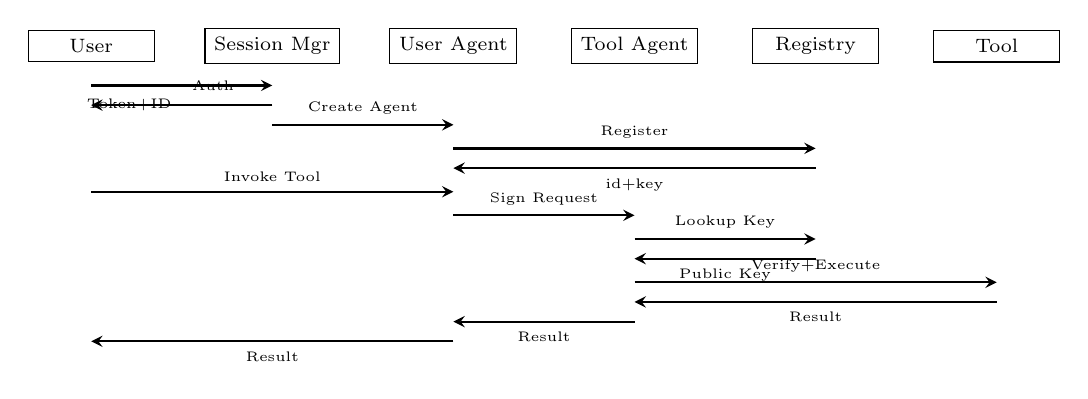
\begin{tikzpicture}[
  node distance=0.2cm,
  entity/.style={rectangle, draw, minimum width=1.6cm, minimum height=0.4cm, font=\scriptsize, align=center},
  arrow/.style={->, thick, >=stealth},
  label/.style={font=\tiny}
]

% Entities at top
\node[entity] (user) at (0,0) {User};
\node[entity] (session) at (2.3,0) {Session Mgr};
\node[entity] (useragent) at (4.6,0) {User Agent};
\node[entity] (toolagent) at (6.9,0) {Tool Agent};
\node[entity] (registry) at (9.2,0) {Registry};
\node[entity] (tool) at (11.5,0) {Tool};

% Authentication phase
\draw[arrow] (0,-0.5) -- node[label, right] {Auth} (2.3,-0.5);
\draw[arrow] (2.3,-0.75) -- node[label, left] {Token+ID} (0,-0.75);

% Agent creation
\draw[arrow] (2.3,-1.0) -- node[label, above] {Create Agent} (4.6,-1.0);

% Registration
\draw[arrow] (4.6,-1.3) -- node[label, above] {Register} (9.2,-1.3);
\draw[arrow] (9.2,-1.55) -- node[label, below] {id+key} (4.6,-1.55);

% Invocation
\draw[arrow] (0,-1.85) -- node[label, above] {Invoke Tool} (4.6,-1.85);
\draw[arrow] (4.6,-2.15) -- node[label, above] {Sign Request} (6.9,-2.15);
\draw[arrow] (6.9,-2.45) -- node[label, above] {Lookup Key} (9.2,-2.45);
\draw[arrow] (9.2,-2.7) -- node[label, below] {Public Key} (6.9,-2.7);

% Verification and execution
\draw[arrow] (6.9,-3.0) -- node[label, above] {Verify+Execute} (11.5,-3.0);
\draw[arrow] (11.5,-3.25) -- node[label, below] {Result} (6.9,-3.25);
\draw[arrow] (6.9,-3.5) -- node[label, below] {Result} (4.6,-3.5);
\draw[arrow] (4.6,-3.75) -- node[label, below] {Result} (0,-3.75);

\end{tikzpicture}
\caption{Registration and invocation flow showing authentication, entity registration, signed invocation, and bidirectional verification.}
\label{fig:registration-invocation}
\end{figure*}

We now introduce authenticated workflows—a protocol-level mechanism that realizes deterministic verification at every agentic boundary crossing.
Against adversaries with capabilities A1-A5 (Section~\ref{sec:threat-model}), authenticated workflows provide four \textbf{cryptographic guarantees} that together achieve security objectives O1-O5:

\textbf{Authenticity} (achieves O1: Integrity): Every accepted invocation is cryptographically linked to the principal that initiated it and the operation being performed. Attackers cannot forge invocations without possessing the principal's private key, binding both WHO (principal) and WHAT (operation).

\textbf{Policy Binding} (achieves O2-O3: Policy Enforcement, Privilege Non-Escalation): The policy governing an operation is cryptographically bound to the invocation, preventing attackers from substituting policies without invalidating signatures.

\textbf{Tamper Evidence} (achieves O4: Context Integrity): Any modification to invocations, context state, or policy bindings is cryptographically detectable through hash chains and sequence numbers.

\textbf{Non-Repudiation} (achieves O5: Accountability): Digital signatures create undeniable proof linking principals to their operations, enabling forensic analysis and compliance verification with tamper-evident audit logs.

As with authenticated system calls \cite{rajagopalan2006,erlingsson2004}, the core idea is conceptually simple: augment every inter-entity invocation with a policy and cryptographic signature that ensures integrity.
{\small
\begin{verbatim}
Invocation = (Args, Policy, MAC)
MAC = Sign(K, Args || Policy)
\end{verbatim}
}
where the Message Authentication Code(MAC) signature cryptographically binds the arguments and policy identifier together using a secret or private key $K$. On the receiving end, verification proceeds in three steps: validate the signature to ensure authenticity and integrity, retrieve and verify the policy binding to prevent substitution, then evaluate whether the operation satisfies policy rules.

\subsection{Design Principles}

Realizing authenticated workflows requires four principles that compose to deliver the cryptographic guarantees:

\textbf{Zero-Trust Identity}: Every entity—agents, tools, data sources, LLMs—possesses unique cryptographic identity (keypair). Even entities in the same process verify each other independently. No implicit trust propagates. We bridge enterprise identity with agent-scale verification: External principals authenticate via enterprise IAM; the runtime propagates these identities as tamper-proof session context. Internally, lightweight ephemeral signatures identify agents, addressing dynamic identity challenges (Section~\ref{sec:policy}).

\textbf{Boundary Verification}: Every inter-entity communication—prompt→LLM, agent→tool, tool→data—requires independent cryptographic verification. Operations carry signatures and policy identifiers; receivers verify signatures using registered public keys, retrieve policies, and evaluate constraints. Verification is transport-agnostic—identical across MCP, LangChain, OpenAI APIs, or custom protocols.

\textbf{Policy Enforcement Points}: PEPs provide independent verification at every boundary—entities cannot verify their own operations. Deployed in-process (linked library) or as sidecars, PEPs verify invocations before execution, providing horizontal scalability, zero-trust verification, tamper resistance, and enforcement independence. This relies on L3 (enforcement integrity).

\textbf{Trustworthy Authenticated Context}: Runtime provides tamper-evident session state such as from~\cite{rajagopalan2025prompts} that ensures integrity including binding operations to session scope (context IDs, session IDs), preventing replay (sequence numbers), detecting tampering (hash-chains), and enabling workflow dependencies (attestations proving prerequisite operations completed).



\noindent\textbf{The Protocol.}
These principles compose into a four-phase protocol that every boundary crossing is an authenticated workflow. Figure~\ref{fig:registration-invocation} shows the complete flow.

\textbf{Registration}: Each entity registers, receiving (agent\_id, keypair). Registration happens at finest granularity—individual tools within agents receive independent (tool\_id, keypair), minimizing blast radius.

\textbf{Invocation}: Caller constructs signed invocation binding operation, arguments, policy, and session context.

\textbf{Verification}: The receiving PEP independently verifies through three stages: (1) signature verification (authenticity + integrity), (2) policy binding verification (prevent substitution), (3) policy evaluation (resource permissions, parameter constraints, attestations). Figure~\ref{fig:verification-flow} details verification.

\textbf{Attestation}: Upon completion, the service signs the result. Context is updated with cryptographically signed attestation proving the operation completed, maintaining Authenticated Context for downstream operations.


Services sign results; callers verify service signatures before accepting results—realizing bidirectional authentication analogous to mutual TLS. This stateless protocol ensures each hop is independently verified without implicit trust propagating through multi-step workflows.



\begin{figure}[t]
\centering
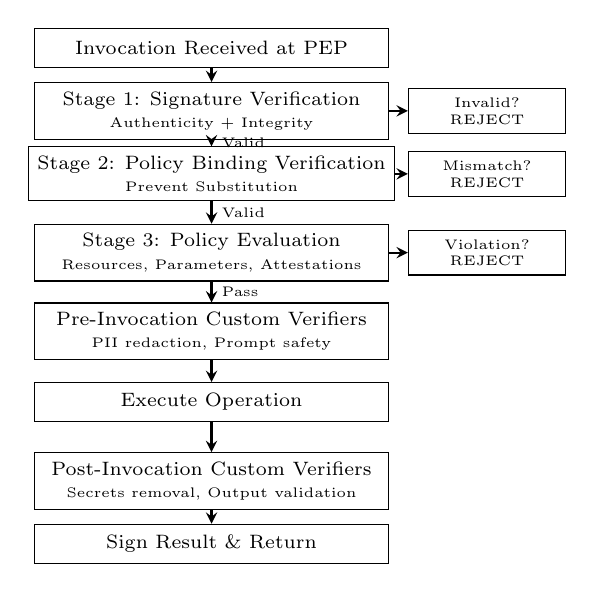
\begin{tikzpicture}[
  node distance=0.4cm,
  box/.style={rectangle, draw, minimum width=4.5cm, minimum height=0.5cm, font=\scriptsize, align=center},
  decision/.style={rectangle, draw, minimum width=2cm, minimum height=0.45cm, font=\tiny, align=center},
  arrow/.style={->, thick, >=stealth}
]

\node[box] (receive) at (0,0) {Invocation Received at PEP};

\node[box] (stage1) at (0,-0.8) {Stage 1: Signature Verification\\{\tiny Authenticity + Integrity}};
\node[decision] (reject1) at (3.5,-0.8) {Invalid?\\REJECT};

\node[box] (stage2) at (0,-1.6) {Stage 2: Policy Binding Verification\\{\tiny Prevent Substitution}};
\node[decision] (reject2) at (3.5,-1.6) {Mismatch?\\REJECT};

\node[box, minimum height=0.7cm] (stage3) at (0,-2.6) {Stage 3: Policy Evaluation\\{\tiny Resources, Parameters, Attestations}};
\node[decision] (reject3) at (3.5,-2.6) {Violation?\\REJECT};

\node[box, minimum height=0.7cm] (pre) at (0,-3.6) {Pre-Invocation Custom Verifiers\\{\tiny PII redaction, Prompt safety}};

\node[box] (execute) at (0,-4.5) {Execute Operation};

\node[box, minimum height=0.7cm] (post) at (0,-5.5) {Post-Invocation Custom Verifiers\\{\tiny Secrets removal, Output validation}};

\node[box] (sign) at (0,-6.3) {Sign Result \& Return};

% Main flow arrows
\draw[arrow] (receive) -- (stage1);
\draw[arrow] (stage1) -- node[right, font=\tiny] {Valid} (stage2);
\draw[arrow] (stage2) -- node[right, font=\tiny] {Valid} (stage3);
\draw[arrow] (stage3) -- node[right, font=\tiny] {Pass} (pre);
\draw[arrow] (pre) -- (execute);
\draw[arrow] (execute) -- (post);
\draw[arrow] (post) -- (sign);

% Reject arrows
\draw[arrow] (stage1.east) -- (reject1.west);
\draw[arrow] (stage2.east) -- (reject2.west);
\draw[arrow] (stage3.east) -- (reject3.west);

\end{tikzpicture}
\caption{PEP verification flow with three-stage cryptographic verification and optional custom verifiers.}
\label{fig:verification-flow}
\end{figure}
\subsection{Verification Flow}

Figure~\ref{fig:verification-flow} shows the verification pipeline—the heart of our integrity claim. The pipeline is always enforced and cannot be escaped: every invocation undergoes cryptographic verification before execution, with receivers independently verifying callers using public keys retrieved from the registry.

\textbf{Policy Construction}: Stage 3 constructs the effective policy independently at the receiver through dual-perspective enforcement. The PEP retrieves organizational policies (company, business unit, team) and resource-specific constraints, computing $P_{\text{eff}} = \text{Intent} \cap \text{Resource}$ (Section~\ref{sec:policy}). The caller's claimed intent is independently verified against resource constraints—callers cannot influence policy evaluation. The intersection algebra (Theorems 1-3) guarantees monotonic restriction: composed policies only narrow permissions, never broaden them.

\textbf{Custom Verifiers}: MAPL's declarative constraints handle resource permissions and parameters, but some security checks require imperative logic on invocation context. Custom verifiers extend policy evaluation with PII detection, SQL injection prevention, prompt safety via LLM classifiers (LLMs as judges), rate limiting, and geolocation checks. Pre-invocation verifiers execute after policy evaluation; post-invocation verifiers process results. Operating on cryptographically verified context, verifiers are trusted code checked in by system administrators, not application developers. Once declared in the verification flow, the PEP enforces their execution—they cannot be bypassed. This provides domain-specific extensibility (HIPAA, GDPR, SOC 2) while maintaining integrity guarantees.

Four production verifiers demonstrate this architecture: (1) MemoryIntegrityVerifier prevents memory poisoning (OWASP LLM01) through rate limiting, protected field enforcement, and cryptographic integrity checks; (2) WorkflowIntegrityVerifier prevents workflow hijacking (OWASP LLM04) by enforcing prerequisite steps and maintaining attestation chains; (3) ToolAuthorizationVerifier prevents tool misuse (OWASP LLM06) via RBAC and dangerous pattern detection (e.g., file\_write→command\_execute); (4) StorageIntegrityVerifier prevents data exfiltration (OWASP LLM02) through path traversal prevention and encryption enforcement. Appendix~\ref{appendix:verifiers} provides implementation details.

This separation is crucial: the core verification pipeline (Stages 1-3: signature verification, policy binding, policy evaluation) provides deterministic guarantees—100\% recall with zero false positives through cryptographic enforcement of MAPL's declarative constraints (Lemmas 1, 4). Custom verifiers (Stages 4-5) are optional administrative extensions that may use heuristics (ML-based PII detection, LLM safety classifiers) and could introduce false positives if misconfigured, but cannot weaken core guarantees—they can only add restrictions, never remove them. Verifiers execute only after cryptographic verification passes, operating on authenticated invocations and tamper-evident state, not unbounded application input. Even if a verifier fails or is compromised, Stages 1-3 still enforce cryptographic integrity and policy constraints. Bypassing verifiers requires corrupting trusted administrator code (L3), not manipulating application logic (A1).

% Table commented out to save space - examples are inline above
% \begin{table}[h]
% \centering
% \caption{Pluggable verifiers for domain-specific compliance}
% \label{tab:verifiers}
% \scriptsize
% \begin{tabular}{@{}p{2.2cm}p{3cm}p{2.2cm}@{}}
% \toprule
% \textbf{Verifier} & \textbf{Function} & \textbf{Compliance} \\
% \midrule
% PII Detection & Redact sensitive fields & HIPAA, GDPR \\
% SQL Guard & Validate queries & OWASP Top 10 \\
% Rate Limiter & Track invocations & DoS prevention \\
% Cmd Injection & Validate parameters & CWE-78 \\
% Context Check & Verify hash chains & SOC 2, ISO 27001 \\
% Geo Residency & Check location & GDPR Art. 44 \\
% \bottomrule
% \end{tabular}
% \end{table}

\noindent\textbf{Security Guarantees.}Against adversaries A1-A5 (Section~\ref{sec:threat-model}), the protocol mechanisms compose into defense-in-depth through four independent cryptographic layers: \textbf{Integrity} (signatures establish authenticity, defeating network attacks A4); \textbf{Authorization} (policy intersection enforces intent—operations must satisfy composed policies even with valid signatures, preventing privilege escalation under application control A1); \textbf{Provenance} (hash chains and sequence numbers make context tamper-evident, defeating content injection A2 and multi-turn manipulation A5); \textbf{Compliance} (custom verifiers add domain-specific validation on cryptographically verified context, providing non-repudiation). Together these achieve security objectives O1-O5.

The protocol provides defense-in-depth: each layer operates independently at each boundary (Lemma 7, Section~\ref{sec:formal-analysis}). Compromising signature verification doesn't bypass policy evaluation; tampering with context doesn't defeat tool PEPs; bypassing one verifier doesn't invalidate cryptographic checks. Section~\ref{sec:formal-analysis} formalizes these independence guarantees.
